\subsection{DLNA}

A \emph{Digital Living Network Alliance} (DLNA) é uma organização composta pelas principais empresas de eletrônicos de consumo, computação e dispositivos móveis. Foi fundada em 2003 e tem como objetivo fornecer orientações para permitir a interoperabilidade entre dispositivos para completar a convergência da indústria digital, levando, dessa forma, inovação, simplicidade e valor para os consumidores~\cite{dlnaoverview}. Tem como visão facilitar a criação, o gerenciamento e o compartilhamento de conteúdo digital (fotos, músicas e vídeos) entre os dispositivos pertencentes à mesma rede~\cite{dlnahdvideostreaming}. Deve permitir, por exemplo~\cite{dlnaoverview}:

\begin{itemize}
	\item Facilmente adquirir, armazenar e acessar música digital a partir de praticamente qualquer lugar da casa;
	\item Facilmente gerenciar, visualizar, imprimir e compartilhar fotos digitais;
	\item Transportar seu conteúdo favorito a partir de qualquer lugar, mesmo que as pontas envolvidas estejam em movimento;
	\item Aproveitar a gravação e reprodução de conteúdo distribuído e multi-usuário.
\end{itemize}

Suas diretrizes destacam casos de uso cuidadosamente construídos para redes domésticas (veja a tabela~\ref{tab:casosdeuso_dlna}), funções adicionais que aumentam a experiência do compartilhamento de conteúdo e doze classes de dispositivos espalhados na categoria "Rede Doméstica e Dispositivos Móveis". A classificação de um dispositivo é feita de tal forma que um único aparelho multifuncional pode possuir diversas categorias diferentes~\cite{dlnahdvideostreaming, dlnaclasses}:

\begin{itemize}
	\item \emph{Home Network Devices}
	\begin{itemize}
		\item \emph{Digital Media Server} (DMS): Esses dispositivos armazenam conteúdo e o torna disponível para \emph{Digital Media Players} (DMP) e \emph{Digital Media Renderes} que estão conectados na rede. Alguns servidores de mídia podem ainda proteger o conteúdo do usuário uma vez que ele tenha sido armazenado. Exemplo: PCs e dispositivos de armazenamento via rede(NAS);
		\item \emph{Digital Media Player} (DMP): Esses dispositivos encontram conteúdo disponibilizados pelos servidores de mídia (DMS) e provêem a capacidade reprodução e renderização de mídia.Exemplos: TVs, aparelhos de som, \emph{home theaters}, monitores sem fio e vídeo games;
		\item \emph{Digital Media Renderer} (DMR): Esses dispositivos tocam conteúdos recebidos do controlador digital de mídia (DMC) que, por sua vez, irá encontrar conteúdo do servidor de mídia digital (DMS). Exemplo: TVs, receptores de áudio ou vídeo, projetores de vídeo e alto-falantes remotos para música;
		\item \emph{Digital Media Controller} (DMC): Esses dispositivos encontram conteúdo em servidores de mídia digital (DMS) e o tocam em renderizadores de mídia digital(DMR). Exemplo: \emph{Tablets}, câmeras digitais com Wi-Fi e PDAs;
		\item \emph{Digital Media Printer} (DMPr): Esses dispositivos provêem serviços de impressão para a rede residencial DLNA. Geralmente, tocadores de mídia digital (DMP) e controladores de mídia digital (DMC) com a capacidade de impressão podem utilizar o DMPr para impressão. Exemplo: Impressoras de foto e multifuncionais conectadas na rede DLNA.
	\end{itemize}
	\item \emph{Mobile Handheld Devices}
	\begin{itemize}
		\item \emph{Mobile Digital Media Server} (M-DMS): Esses dispositivos sem fio armazenam conteúdo e o tornam disponível para tocadores de mídia digital que tenham acesso à rede sem fio ou com fio (M-DMP), renderizadores de mídia digital (DMR) e impressoras de mídia digital (DMPr). Exemplo: telefones portáteis e tocadores portáteis de música;
		\item \emph{Mobile Digital Media Player} (M-DMP): Esses dispositivos sem fio encontram e tocam conteúdo de um servidor de mídia digital (DMS) ou servidor móvel de mídia digital (M-DMS). Exemplo: telefones portáteis, \emph{tablets} projetados para visualização de conteúdo multimídia;
		\item \emph{Mobile Digital Media Uploader} (M-DMU): Esses dispositivos sem fio enviam conteúdo para um servidor digital de de mídia (DMS) ou para um servidor móvel de mídia digital (M-DMS). Exemplo: câmeras digitais, e telefones portáteis;
		\item \emph{Mobile Digital Media Downloader} (M-DMD): Esses dispositivos sem fio encontram e armazenam conteúdo de um servidor de mídia digital (DMS) ou de um servidor móvel de mídia digital (M-DMS). Exemplo: tocadores de música e telefones portáteis;
		\item \emph{Mobile Digital Media Controller} (M-DMC): Esses dispositivos encontram conteúdo em um servidor digital de mídia(DMS) ou em um servidor móvel de mídia digital (M-DMS) e o envia para renderizadores de mídia digital(DMR). Exemplo: telefones portáteis e PDAs.
	\end{itemize}
	\item \emph{Home Infrastructure Devices}
	\begin{itemize}
		\item \emph{Mobile Network Connectivity Function} (M-NCF): Esses dispositivos provêem uma ligação entre a conectividade de rede de dispositivos móveis portáteis e conectividade de rede residencial;
		\item \emph{Media Interoperability Unit} (MIU): Esses dispositivos provêem transformação de conteúdo entre formatos de mídia necessários para uma rede residencial ou para dispositivos móveis portáteis.
	\end{itemize}
\end{itemize}

\begin{comment}
\begin{table}
	\begin{center}
		\begin{tabular}{llll}
		\hline
		\textbf{Classe} & \textbf{Categoria} & \textbf{Descrição} & \textbf{Exemplo}						\\
		\hline
		\hline
		Mobile Network Connectivity Function (M-NCF) & \multirow{2}{*}{Home Infrastructure Devices} &  & \\
		\hline
		Media Interoperability Unit (MIU) & &  & \\
		\hline
		\end{tabular}
	\end{center}
	\caption{Classes DLNA~\cite{}.}
	\label{tab:classes_dlna}
\end{table}
\end{comment}

Imagine, por exemplo, uma situação hipotética em que uma pessoa deseja compartilhar um pequeno vídeo com seus amigos a partir de seu celular. A fim de exibir esse vídeo em sua TV widescreen na sua sala de estar, ela necessita, primeiramente, envia-lo para seu próprio email. Em seguida, deve ligar seu PC, fazer o download do vídeo e salvá-lo em um \emph{pendrive} ou cartão de memória. Posteriormente, deve ligá-lo na TV ou em um receptor digital e, então, utilizar a interface do dispositivo para localizar o vídeo e exibi-lo~\cite{dlnahdvideostreaming}.

Além de interromper a conversa, esse tipo de processo de transferência de conteúdo simplesmente consome muito tempo, mesmo quando ocorre sem problemas. Como resultado, a partilha informal de vídeo em múltiplas telas não é visto muitas vezes como uma opção razoável~\cite{dlnahdvideostreaming}.

\begin{figure}[ht]
	\center
	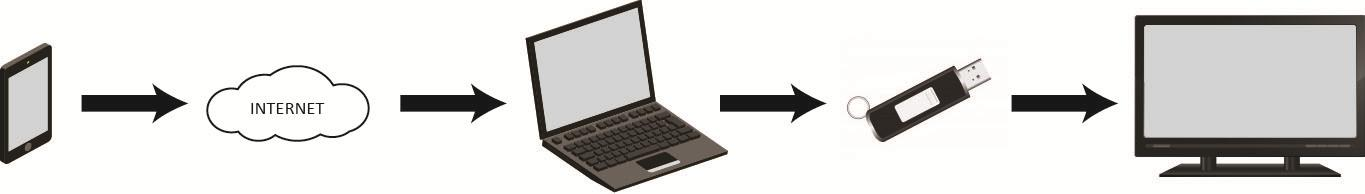
\includegraphics[scale=0.3]{imagens/dlna1}
	\caption{A exibição de um vídeo ou foto de um celular em uma TV envolve tal processo tradicional, tedioso e demorado que os consumidores raramente farão.}
	\label{fig:traditionalProccess}
\end{figure}

Este é o valor da proposição que o DLNA oferece aos seus consumidores: a partilha contínua e sem esforço de conteúdo digital. Produtos projetados seguindo as diretrizes DLNA estabelecidas para compartilhar vídeo em apenas um único passo: a transmissão de uma cópia do vídeo do telefone sem fio para a TV. O consumidor pode até mesmo congelar o vídeo usando um "controle remoto" do menu no telefone, bem como \emph{fast-forward} e reproduzir o vídeo~\cite{dlnahdvideostreaming}.

\begin{figure}[ht]
	\center
	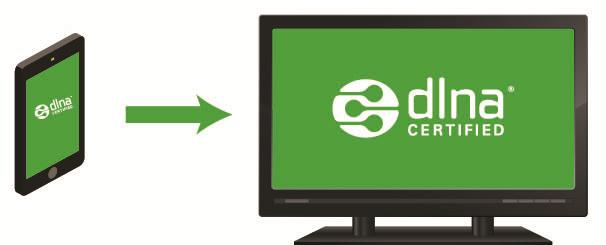
\includegraphics[scale=0.3]{imagens/dlna2}
	\caption{O valor da proposição do DLNA é o compartilhamento transparente e fácil de conteúdo, permitindo que os consumidores enviem uma cópia de um vídeo ou fotos diretamente para a TV em uma única etapa.}
	\label{fig:dlnaProccess}
\end{figure}

Em suma, o DLNA pode ser visto como uma coleção de padrões abertos que definem como uma rede residencial interage em todos os seus níveis, ou seja, além de definir como os diferentes padrões irão interoperar e como os dados serão tratados em cada nível, ele também reduz o número de padrões que um dispositivo deve suportar.

\begin{table}
	\begin{center}
		\begin{tabular}{rl}
		\hline
		\textbf{Casos de Uso} & \textbf{Exemplo}																\\
		\hline
		Enviar & Transferir vídeos ou imagens capturadas em uma câmera digital ou celular para um computador.	\\
		\hline
		Empurrar & Exibir vídeos ou imagens capturadas em uma câmera digital ou celular diretamente em uma TV sem intermédio de um computador. \\
		\hline
		Localizar e Reproduzir ou "Reproduzir em..."" & Utiliza um celular para localizar uma música ou vídeo armazenados em um computador, unidade de disco externa ou um dispositivo \emph{Network-Attached Storage} (NAS) e transferi-lo, via \emph{stream} ou não, para reprodução. \\
		\hline
		Puxar e imprimir ou "Imprimir em..." & Visualizar na TV uma foto armazenada em um servidor de mídia e imprimi-la utilizando uma impressora em rede. \\
		\hline
		\end{tabular}
	\end{center}
	\caption{Exemplos de casos de uso~\cite{dlnahdvideostreaming}.}
	\label{tab:casosdeuso_dlna}
\end{table}

\begin{table}
	\begin{center}
		\begin{tabular}{rll}
		\hline
		\textbf{Camada} & \textbf{Função definida} & \textbf{Padrões}				\\
		\hline
		Transmissão Protegida & Como um conteúdo comercial está protegido em uma rede doméstica. & DTCP/IP \\
		\hline
		Formatos de Mídia & Como um conteúdo de mídia está codificado e identificado para interoperabilidade. & MPEG2, MPEG4, AVC/H.264, LPCM, MP3, AAC LC, JPEG, XHTML-Print- \\
		\hline
		Transporte de Mídia & Como um conteúdo de mídia é transferido. & HTTP, Quality of Service \\
		\hline
		Gerência de Mídia & Como um conteúdo de mídia é identificado, gerenciado e distribuído. & UPnP AV 1.0, UPnP Print Enhanced 1.0 \\
		\hline
		Descoberta e Controle & Como dispositivos se descobrem e se controlam um ao outro. & UPnP Device Architecture 1.0 \\
		\hline
		Redes IP & \multirow{2}{*}{Como dispositivos com e sem fio fisicamente se conectam e se comunicam.} & IPv4 Protocol Suite \\
		Conectividade & & Wired: Ethernet 802.3, MoCAWireless: Wi-Fi 802.11, Wi-Fi Protected Setup \\
		\hline
		\end{tabular}
	\end{center}
	\caption{Camadas padrões DLNA~\cite{dlnahdvideostreaming}.}
	\label{tab:camadaspadroes_dlna}
\end{table}
